\documentclass[12pt,a4paper]{article}

\usepackage[a4paper,margin=1in]{geometry}
\usepackage{graphicx}
\usepackage{booktabs}
\usepackage{amsmath,amssymb}
\usepackage{float}
\usepackage{hyperref}
\usepackage{xcolor}
\usepackage{listings}
\usepackage{enumitem}
\usepackage{fancyhdr}
\usepackage{longtable}

\hypersetup{colorlinks=true,linkcolor=blue,urlcolor=blue}

\pagestyle{fancy}
\fancyhf{}
\lhead{ICS1512}
\rhead{Machine Learning Algorithms Laboratory}
\cfoot{\thepage}

\lstset{
language=Python,
basicstyle=\ttfamily\small,
numbers=left,
frame=single,
breaklines=true,
showstringspaces=false
}

\begin{document}

\begin{tabular}{|p{4cm}|p{11cm}|}
\hline
Experiment No. & 3 \\ \hline
Experiment Title & Regression Analysis using Linear and Regularized Models\footnotemark\\ \hline
Student Name & Simiyon Vinscent Samuel L \\ \hline
Register Number & 3122247001062 \\ \hline
Faculty & Dr. Poreddy Ajay Kumar Reddy \\ \hline
Submission Date & August 2, 2026 \\ \hline
\end{tabular}
\footnotetext{\textbf{GitHub Repository: }\url{https://github.com/blackscythe123/Machine-Learning-course}}

\section{Objective}
To implement linear and regularized regression models for predicting a continuous target
variable (the sanctioned loan amount), evaluate their performance using multiple metrics,
visualize model behaviour, and analyze overfitting, underfitting and bias--variance
characteristics.

\section{Problem Statement}
Given the Kaggle / Analytics Vidhya loan prediction dataset (592 applicants after dropping
rows with a missing target, 10 raw features covering applicant demographics, income and
credit history), the task is to predict the continuous \texttt{LoanAmount} sanctioned to
each applicant, a supervised \textbf{regression} problem. Four linear model families
(Linear, Ridge, Lasso and Elastic Net Regression) are trained and compared. Beyond finding
the best-performing model, the goal is to understand how regularization strength and
penalty type (L1 vs.\ L2) shape the bias--variance trade-off on this small, skewed dataset.

\section{Dataset Description}
\begin{longtable}{|p{6cm}|p{8cm}|}
\hline
Dataset Name & Loan Prediction Dataset \\ \hline
Dataset Source & Kaggle / Analytics Vidhya Loan Prediction Practice Problem \\ \hline
Number of Samples (after dropping rows with missing target) & 592 \\ \hline
Target Variable & \texttt{LoanAmount} (continuous, in thousands) \\ \hline
Raw Feature Count & 10 (5 numeric, 5 categorical) \\ \hline
Encoded Feature Count & 11 (after one-hot encoding of categorical variables) \\ \hline
Missing Values (raw) & Gender: 13, Married: 3, Dependents: 15, Self\_Employed: 32,
LoanAmount: 22, Loan\_Amount\_Term: 14, Credit\_History: 50 \\ \hline
Train-Test Split & 80\% train (473 samples) / 20\% test (119 samples) \\ \hline
\end{longtable}

\section{Exploratory Data Analysis}

\subsection*{Target Variable Distribution}
\begin{figure}[H]
\centering
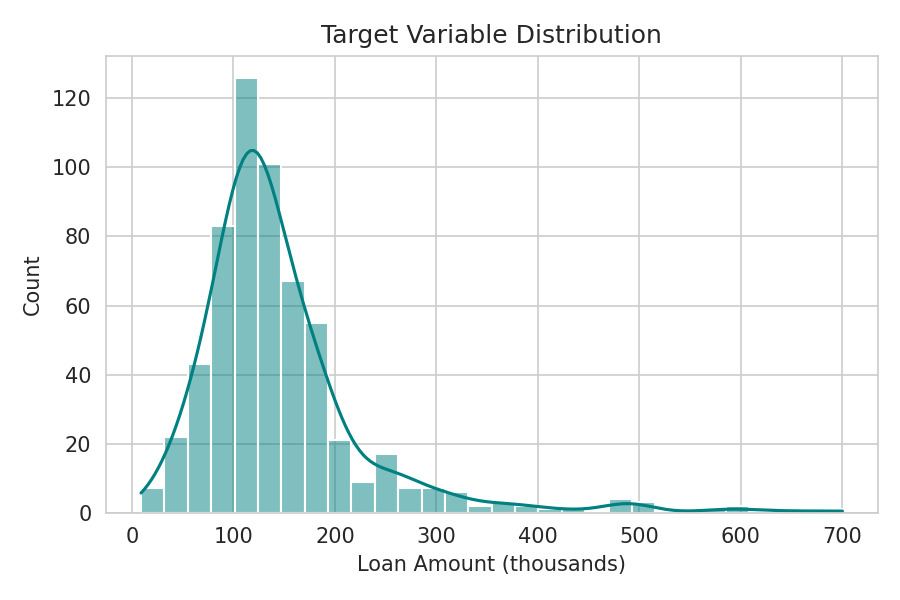
\includegraphics[width=0.6\linewidth]{figures/01_target_distribution.png}
\caption{Distribution of the sanctioned loan amount.}
\end{figure}
\textbf{Inference:} \texttt{LoanAmount} is strongly right-skewed, with most applicants
sanctioned amounts in the 100--150 (thousand) range and a long tail of a few large loans.
This skew is one reason plain linear models struggle to fit the tail well and partly
explains the relatively modest $R^2$ obtained below.

\subsection*{Feature vs. Target Scatter Plots}
\begin{figure}[H]
\centering
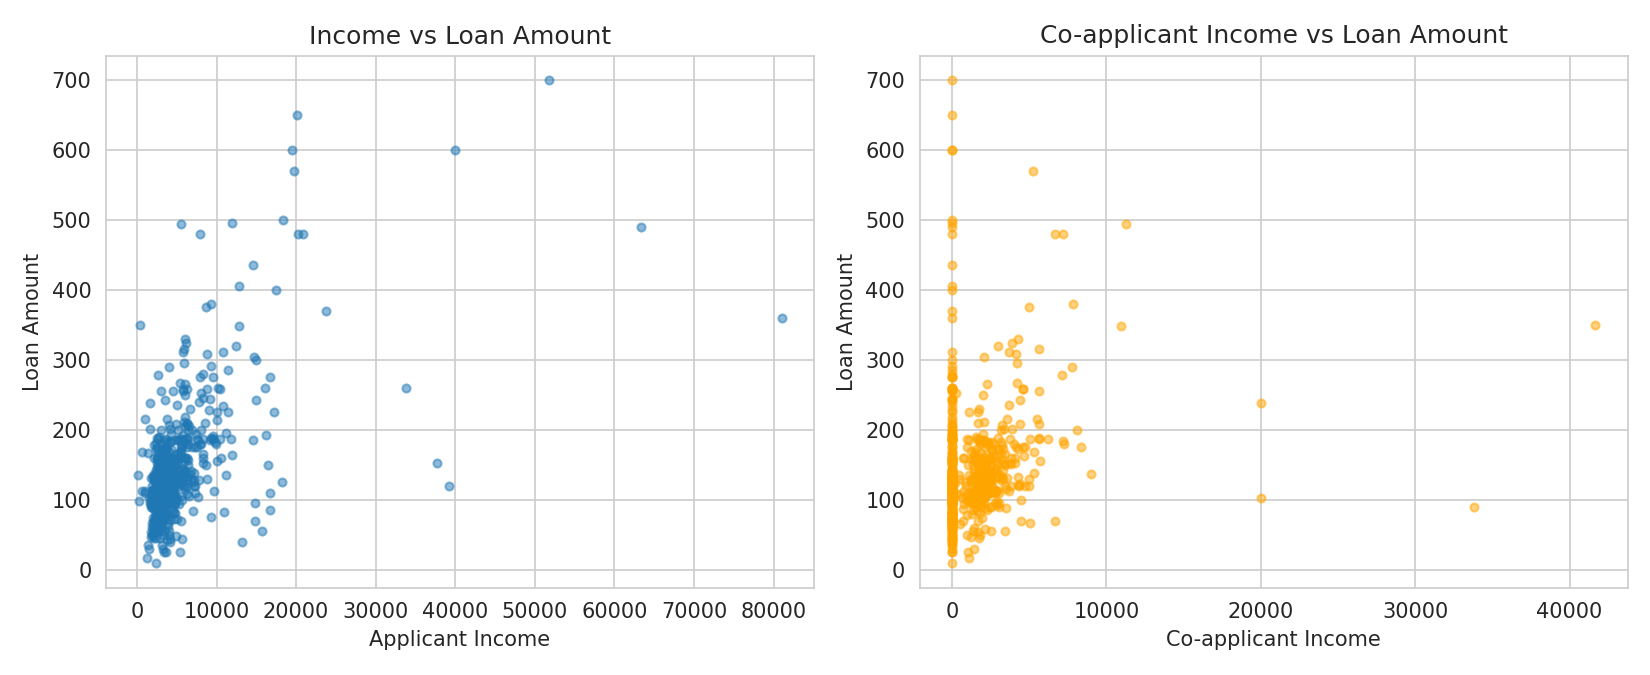
\includegraphics[width=0.95\linewidth]{figures/02_feature_vs_target.png}
\caption{Applicant income and co-applicant income vs.\ loan amount.}
\end{figure}
\textbf{Inference:} Applicant income shows a weak positive trend with loan amount, with
substantial scatter, particularly a handful of high-income outliers that pull the linear
fit without necessarily corresponding to proportionally larger loans. This weak, noisy
relationship anticipates the limited predictive power ($R^2 \approx 0.1$--$0.4$)
observed for every model.

\section{Data Preprocessing}
\begin{itemize}
\item \textbf{Target rows with missing \texttt{LoanAmount}} (22 rows) were dropped, since
imputing the prediction target itself would bias evaluation.
\item \textbf{Categorical missing values} (\texttt{Gender}, \texttt{Married},
\texttt{Dependents}, \texttt{Self\_Employed}) were imputed with the column mode.
\item \textbf{Numeric missing values} (\texttt{Loan\_Amount\_Term}, \texttt{Credit\_History})
were imputed with the column median, which is robust to the outliers visible in these
columns.
\item \textbf{\texttt{Dependents}} category ``3+'' was mapped to the integer 3 so the
column could be treated as ordinal/numeric.
\item \textbf{Categorical encoding:} \texttt{Gender}, \texttt{Married}, \texttt{Education},
\texttt{Self\_Employed} and \texttt{Property\_Area} were one-hot encoded
(\texttt{drop\_first=True} to avoid the dummy-variable trap).
\item \textbf{Feature scaling:} All 11 encoded features were standardized
(\texttt{StandardScaler}, fit on the training split only) so that the regularization
penalty in Ridge/Lasso/Elastic Net is applied fairly across features of different
natural scale (income figures span thousands; \texttt{Credit\_History} is 0/1).
\end{itemize}

\section{Machine Learning Algorithm}
Four linear model families were trained and compared:
\begin{itemize}
\item \textbf{Linear Regression} -- ordinary least squares, no penalty, serves as the
baseline.
\item \textbf{Ridge Regression} -- L2 penalty $\lambda\sum w_i^2$, shrinks coefficients
smoothly.
\item \textbf{Lasso Regression} -- L1 penalty $\lambda\sum|w_i|$, can shrink coefficients
exactly to zero (feature selection).
\item \textbf{Elastic Net} -- combines L1 and L2 penalties via the \texttt{l1\_ratio}
parameter.
\end{itemize}
All four minimize a squared-error loss; the three regularized variants add a penalty term
controlled by $\alpha$ (and, for Elastic Net, the L1/L2 mixing ratio \texttt{l1\_ratio})
that shrinks the coefficient vector $w$ toward zero.
\textbf{Advantages:} Fast to train (closed-form or convex optimization), directly
interpretable coefficients, and, for Ridge/Lasso/Elastic Net, a single regularization
strength parameter gives explicit control over overfitting.
\textbf{Limitations:} All four assume a linear relationship between features and target
and cannot capture non-linear or interaction effects unless such terms are engineered
explicitly; Lasso's hard feature elimination can also discard features that carry a small
but real signal.

\section{Experimental Setup}
\begin{tabular}{ll}
\toprule
Python Version & 3.12.3 \\
Scikit-Learn Version & 1.8.0 \\
IDE & Jupyter Notebook \\
Operating System & Windows 11 \\
Hardware & Intel Core Ultra 9, NVIDIA RTX 5060 \\
\bottomrule
\end{tabular}

\section{Hyperparameter Selection}
Ridge, Lasso and Elastic Net were each tuned with \texttt{GridSearchCV} using 5-fold
\texttt{KFold} cross-validation, optimizing $R^2$, over the search space specified in the
lab manual.

\subsection*{Table 1: Hyperparameter Tuning Summary}
\begin{tabular}{llc}
\toprule
Model & Best Parameters & Best CV $R^2$ \\
\midrule
Ridge Regression & $\alpha=100$ & 0.3714 \\
Lasso Regression & $\alpha=10$ & 0.3311 \\
Elastic Net Regression & $\alpha=1$, $l1\_ratio=0.8$ & \textbf{0.3710} \\
\bottomrule
\end{tabular}

\section{Results}

\subsection*{Table 2: Cross-Validation Performance ($K=5$, Training Set)}
\begin{tabular}{lcccc}
\toprule
Model & MAE & MSE & RMSE & $R^2$ \\
\midrule
Linear Regression & 43.06 & 5506.90 & 74.21 & 0.3110 \\
Ridge Regression & 44.07 & 4932.95 & 70.23 & \textbf{0.3714} \\
Lasso Regression & 46.23 & 5281.51 & 72.67 & 0.3311 \\
Elastic Net Regression & \textbf{43.85} & \textbf{4939.55} & \textbf{70.28} & 0.3710 \\
\bottomrule
\end{tabular}

\subsection*{Table 3: Test Set Performance}
\begin{tabular}{lcccc}
\toprule
Model & MAE & MSE & RMSE & $R^2$ \\
\midrule
Linear Regression & \textbf{36.52} & \textbf{3352.43} & 57.90 & 0.0906 \\
Ridge Regression & 37.37 & 3175.95 & 56.36 & 0.1385 \\
Lasso Regression & 37.80 & 3176.80 & 56.36 & 0.1382 \\
Elastic Net Regression & 37.32 & 3163.59 & \textbf{56.25} & \textbf{0.1418} \\
\bottomrule
\end{tabular}

\subsection*{Table 4: Coefficient Comparison (Top 8 Features)}
\begin{tabular}{lcccc}
\toprule
Feature & Linear & Ridge & Lasso & Elastic Net \\
\midrule
ApplicantIncome & 54.03 & 43.88 & 44.98 & 43.76 \\
CoapplicantIncome & 22.30 & 17.22 & 11.79 & 16.76 \\
Married\_Yes & 9.43 & 7.87 & 1.74 & 7.51 \\
Loan\_Amount\_Term & 7.71 & 5.64 & 0.00 & 4.98 \\
Self\_Employed\_Yes & 6.46 & 6.18 & 0.00 & 5.66 \\
Education\_Not Graduate & $-$6.38 & $-$6.81 & 0.00 & $-$6.23 \\
Property\_Area\_Urban & $-$5.47 & $-$4.12 & 0.00 & $-$3.01 \\
Dependents & 4.98 & 5.72 & 0.00 & 5.28 \\
\bottomrule
\end{tabular}

\section{Result Visualization}

\subsection*{Predicted vs. Actual Values}
\begin{figure}[H]
\centering
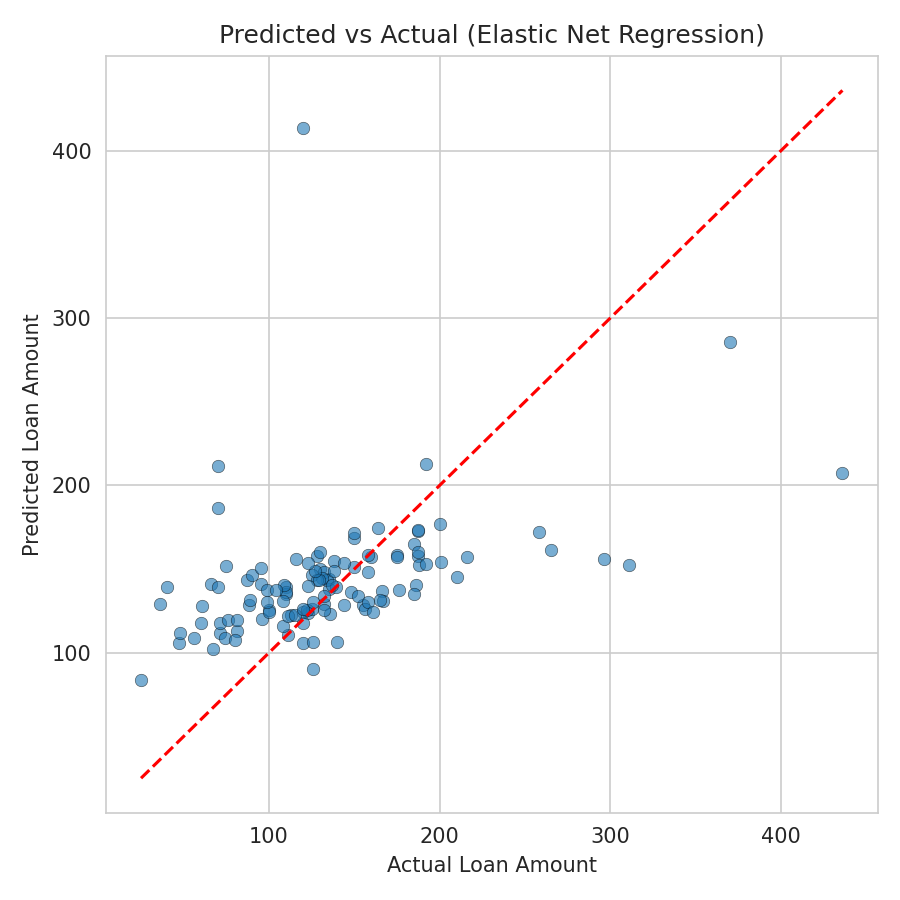
\includegraphics[width=0.55\linewidth]{figures/03_predicted_vs_actual.png}
\caption{Predicted vs.\ actual loan amount for the best test-set model (Elastic Net).}
\end{figure}
\textbf{Inference:} Points cluster loosely around the diagonal for typical loan amounts
but the model systematically under-predicts the largest loans, visible as points falling
well below the red reference line at the top-right, a direct consequence of the
right-skewed target distribution and the linear models' inability to represent the
non-linear tail behaviour.

\subsection*{Residual Plot}
\begin{figure}[H]
\centering
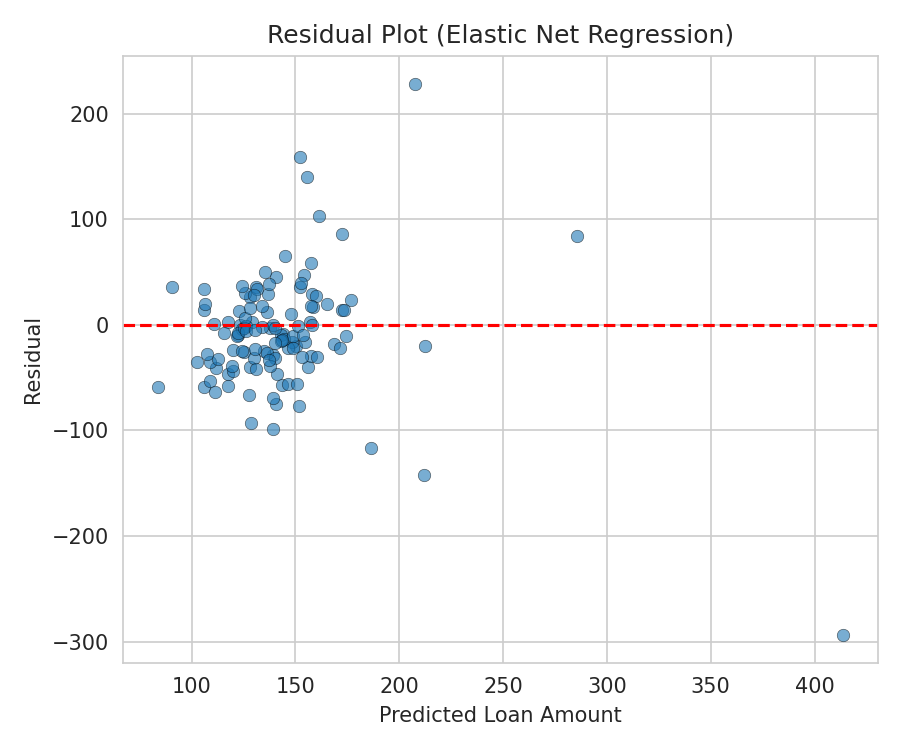
\includegraphics[width=0.55\linewidth]{figures/04_residual_plot.png}
\caption{Residuals vs.\ predicted values (Elastic Net).}
\end{figure}
\textbf{Inference:} Residuals fan out and become more positive (under-prediction) as the
predicted loan amount increases, a classic sign of heteroscedasticity linked to the
skewed target; a log-transform of \texttt{LoanAmount} would likely stabilize this
variance and is a natural next step beyond the scope of this experiment.

\subsection*{Training vs. Validation Error}
\begin{figure}[H]
\centering
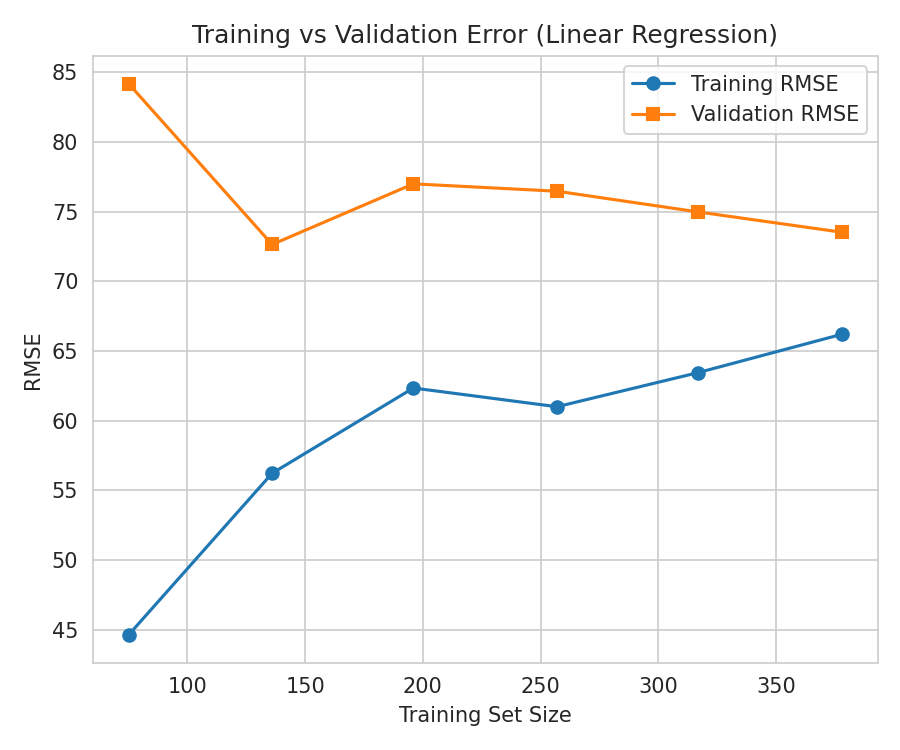
\includegraphics[width=0.6\linewidth]{figures/05_train_val_error.png}
\caption{Training vs.\ validation RMSE as training set size increases (Linear
Regression).}
\end{figure}
\textbf{Inference:} Both curves converge toward a similar, fairly high RMSE as the
training set grows, with only a small persistent gap. This pattern is typical of
\textbf{high bias, low variance}: the linear model is not overfitting (the gap is
small), but it is also not able to drive validation error much lower, meaning more data
alone would not help much; more informative features or a non-linear model would.

\subsection*{Coefficient Comparison}
\begin{figure}[H]
\centering
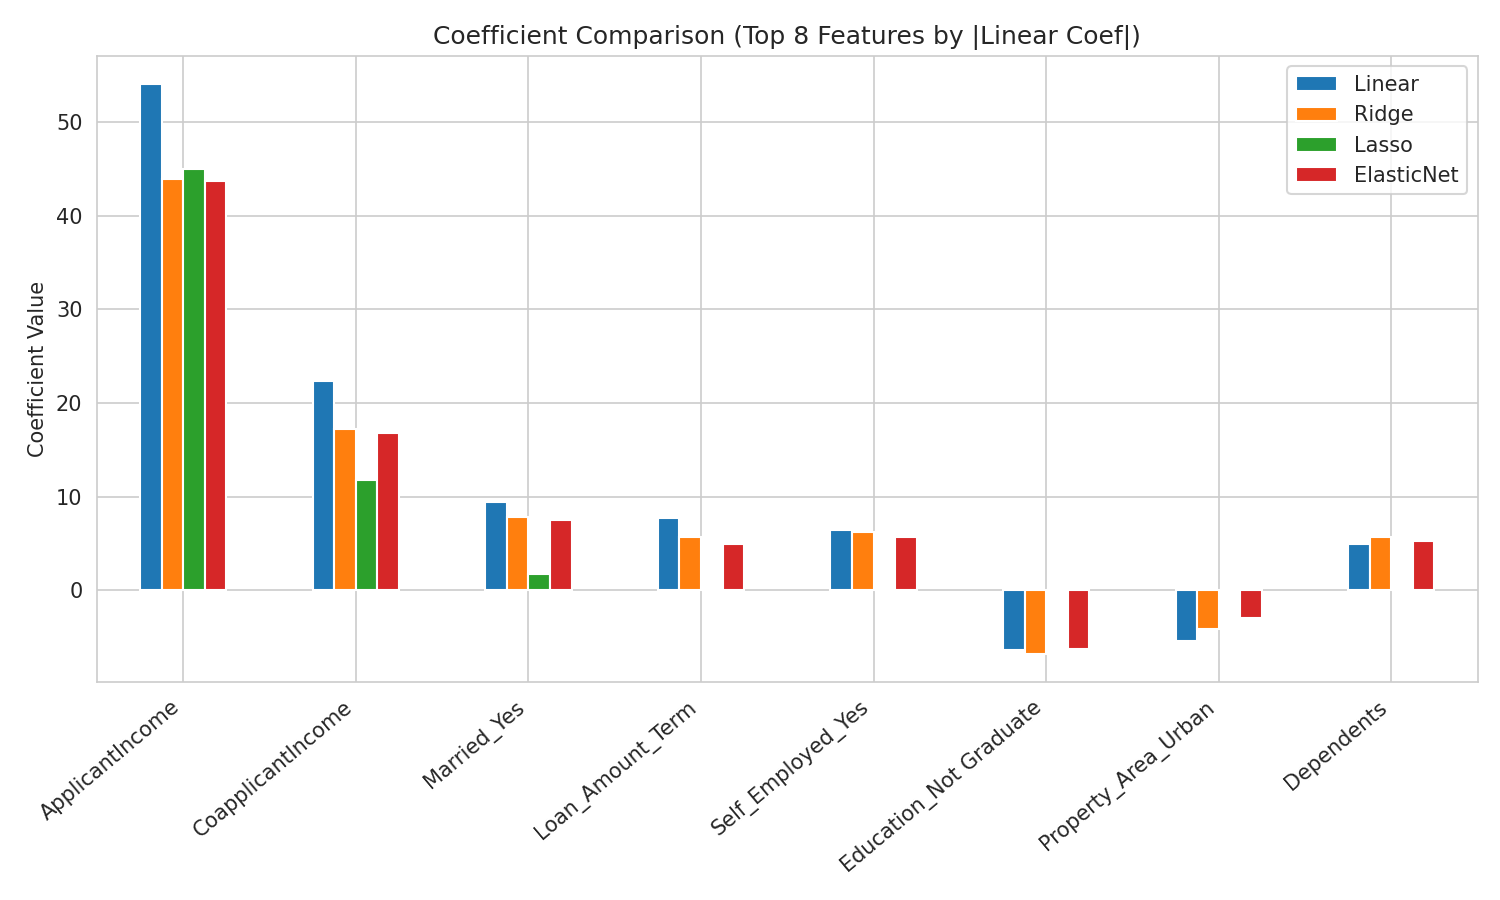
\includegraphics[width=0.95\linewidth]{figures/06_coefficient_comparison.png}
\caption{Coefficient magnitudes for the top 8 features, across all four models.}
\end{figure}
\textbf{Inference:} \texttt{ApplicantIncome} and \texttt{CoapplicantIncome} carry by far
the largest coefficients in every model, confirming they are the dominant predictors.
Lasso drives \texttt{Loan\_Amount\_Term}, \texttt{Self\_Employed\_Yes},
\texttt{Education\_Not Graduate}, \texttt{Property\_Area\_Urban} and \texttt{Dependents}
coefficients to exactly zero at its tuned $\alpha=10$, performing genuine feature
selection, while Ridge and Elastic Net shrink these same coefficients toward zero
without eliminating them.

\subsection*{Test Set Performance Comparison}
\begin{figure}[H]
\centering
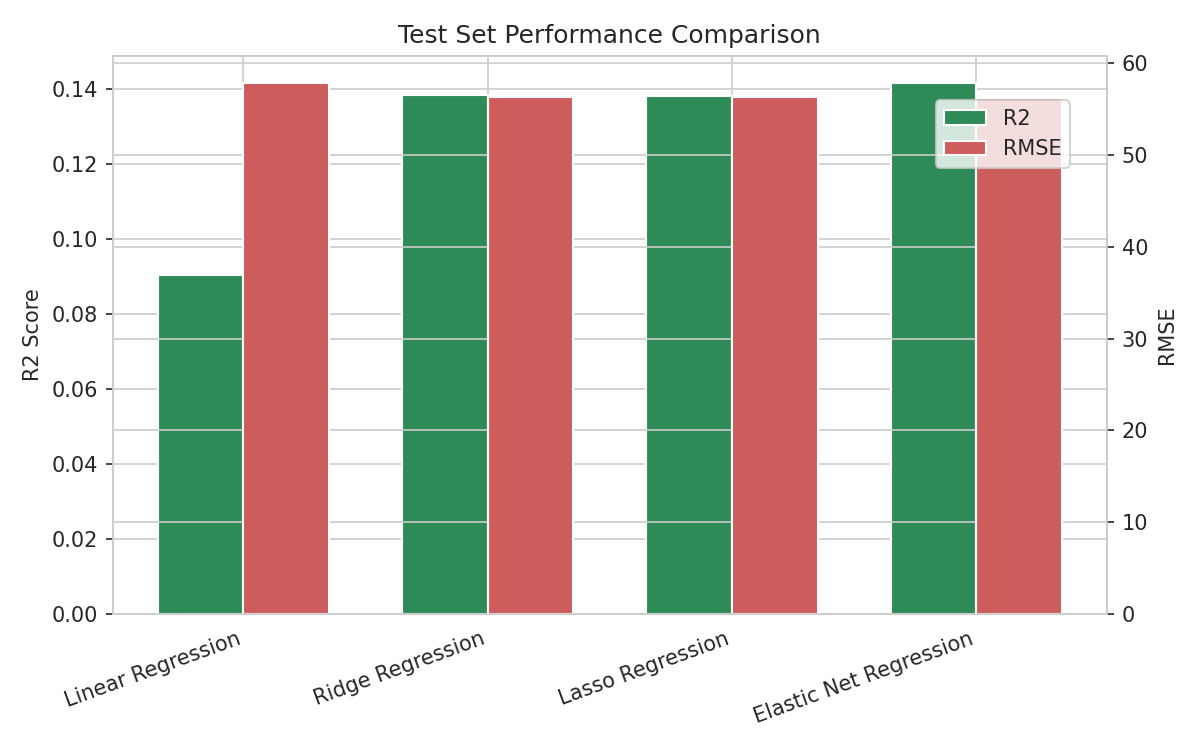
\includegraphics[width=0.75\linewidth]{figures/07_test_performance_comparison.png}
\caption{$R^2$ and RMSE for all four models on the held-out test set.}
\end{figure}

\section{Discussion}

\subsection*{Overfitting and Underfitting Analysis}
Every model's cross-validation $R^2$ (0.31--0.37, computed on the training folds) is
noticeably \emph{higher} than its held-out test $R^2$ (0.09--0.14). At first glance this
looks like overfitting, but the gap here is better explained by the small dataset size
(592 samples total, only 119 in the held-out test set): with so few test points, the
$R^2$ estimate itself has high variance, and a handful of large, hard-to-predict loan
amounts landing in the test split can noticeably drag test $R^2$ down independent of
model quality. The learning curve (Figure 5) supports this reading: training and
validation RMSE are close together and both plateau, which is the signature of
\textbf{high bias / underfitting}, not high variance / overfitting. Regularization
strength reflects this: the best-performing models (Ridge and Elastic Net) both selected
comparatively \emph{large} $\alpha$, i.e.\ strong regularization, but the improvement
over unregularized Linear Regression is modest (CV $R^2$ 0.311 $\to$ 0.371), consistent
with a model that is bias-limited rather than variance-limited. After tuning,
generalization (as measured by the CV/test $R^2$ gap for Ridge and Elastic Net) is not
meaningfully better than the untuned baseline, reinforcing that the ceiling here is the
information content of the available features, not overfitting.

\subsection*{Bias-Variance Analysis}
\begin{itemize}
\item \textbf{Linear Regression} sits at the high-bias end: it has zero built-in
capacity to ignore noisy or weak features, so every feature (including
\texttt{Loan\_Amount\_Term} and \texttt{Dependents}, whose true effect is likely small)
gets a non-zero coefficient, but its overall explanatory power is still limited by the
weak linear relationship between features and target.
\item \textbf{Ridge and Elastic Net} reduce variance by shrinking all coefficients
toward zero, which is why they achieve the best cross-validated $R^2$; they trade a
small amount of bias for a larger reduction in variance, the classic favourable
bias-variance trade at moderate regularization strength.
\item \textbf{Lasso's feature sparsity effect} is the most visible in Table 4: at its
tuned $\alpha=10$, five of the eight shown coefficients are driven to exactly zero,
leaving only \texttt{ApplicantIncome}, \texttt{CoapplicantIncome} and a small
\texttt{Married\_Yes} effect. This aggressive sparsity slightly \emph{increases} bias
relative to Ridge (Lasso's CV $R^2$ of 0.331 is the lowest of the three regularized
models), suggesting that some of the zeroed-out features (e.g.\ \texttt{Credit\_History}
related dummies, \texttt{Education}) do carry a small amount of real signal that Ridge
and Elastic Net retain.
\end{itemize}

\section{Conclusion}
Elastic Net Regression gave the best held-out test performance (RMSE 56.25, $R^2$
0.1418) and was statistically tied with Ridge for the best cross-validated $R^2$
(0.3710 vs.\ 0.3714), while offering Lasso-like sparsity on some features through its
$l1\_ratio=0.8$ setting. Given the small dataset and the loan amount's skewed
distribution, none of the four linear models achieves strong absolute predictive power:
this reflects a genuine ceiling in the available features (largely income and
demographic fields) rather than a modelling failure, and is itself a useful finding:
practitioners working with this dataset should expect that accurately predicting the
exact sanctioned amount requires additional features (e.g.\ property value, existing
liabilities) beyond what is provided here. Among the four models, \textbf{Elastic Net} is
recommended as the best trade-off between accuracy, coefficient interpretability and
robustness to the correlated income features, since it inherits Ridge's stability while
still zeroing out the least useful predictors.

\section{References}
\begin{enumerate}
\item Scikit-learn Developers, ``Linear Models,'' Scikit-learn Documentation. [Online].
Available: \url{https://scikit-learn.org/stable/modules/linear_model.html}
\item Scikit-learn Developers, ``Tuning the hyper-parameters of an estimator,''
Scikit-learn Documentation. [Online]. Available:
\url{https://scikit-learn.org/stable/modules/grid_search.html}
\item Loan Prediction Dataset, Analytics Vidhya / Kaggle Loan Prediction Practice
Problem.
\end{enumerate}

\end{document}
